% \documentclass[english, draft]{article}
\documentclass[english]{article}

\usepackage{geometry}
\usepackage{float}
\usepackage[utf8]{inputenc}
\usepackage[backend=biber,style= authoryear]{biblatex}
\usepackage[english]{babel}
\usepackage{csquotes}
\usepackage{graphicx}
\usepackage{subcaption}
\usepackage{booktabs}
\usepackage{xargs}
\usepackage[pdftex,dvipsnames,table]{xcolor}
\usepackage{bbold}
\usepackage{diagbox}

\graphicspath{{./resources/images}}
\addbibresource{../articles.bib}
\addbibresource{../manual.bib}

\geometry{a4paper, total={165mm,257mm}, left=15mm, top=20mm,}

\begin{document}
\pagenumbering{arabic}

\begin{abstract}

\end{abstract}

\section{Background}
European grapevine (Vitis vinifera L.) is one of the most economically and widespread worldwide crop. Around 33 of the  10.000 varieties,  cover 50\% of the world's vineyard surface (OIV, 2017).
Grapevine faces numerous pathogens and one of the most damaging diseases is downy mildew, caused by the oomycete Plasmopara viticola. This pathogen is endemic to the North America and was introduced into Europe around the 1870s (Gessler et al., 2011., Fontaine et al., 2021). All the Vitis vinifiera varieties are susceptible to the pathogen and the current strategy to control the disease  relies on the massive applications of fungicides and which are potentially harmful for the humans and the environment. Long -lasting breeding programs have been conducted to introgress resistance from wild Vitis species into elite resistant varieties (Merdinoglu et al., 2018; Töpfer \& Trapp, 2022). According to Possamai \& Wiedemann-Merdinoglu, (2022), more than 30 resistance genetic loci or Rpv (Resistance to Plasmopara viticola), have been already identified in grapevine and the majority of them confer a visual partial resistance defined by various levels of sporulation and  necrosis. The analysis of macroscopic phenotypes of the disease have been implemented by using several variables such as severity, incidence, spores count. Therefore, the use of the semi-quantitative OIV452-1 scale was frequently used assessing both sporulation and necrosis.

\section{Material and Method}

The proposed plant method includes four main items: (i) The imaging acquisition system developed to acquire images of \textit{Vitis} leaf discs infected with \textit{Plasmopara viticola} used to create (ii) the dataset, which needs to benefit from (iii) pre-processing before investigating (iv) various approaches for the quantification of the interaction between the plant and the pathogen.

\subsection{Imaging system}
Different RGB cameras have been used over the years to acquire plate images, each one containing twelve leaf discs, from the top view as illustrated in Fig.~\ref{fig:vegoia}. Two overhead spots are used to remove shadows that could hinder image processing tasks. As a consequence of using different setups the images have varied framings and exposures.

\subsection{Dataset}
\paragraph{}
Experiments to evaluate the resistance of various \textit{Vitis} species to various strains of \textit{P. viticola} with image acquisitions have been performed at INRAE center Grand Est Colmar since 2012. After infection leaf discs were manually annotated using a binocular magnifying glass and imaged with an RGB camera the day of inoculation and at 3, 4, 5 and 6 DPIs, annotations and image names were recorded using Microsoft Excel files to keep track of the experiments. Annotations consisted of a score for \cite{} OIV 452-1. At the start of this project 75k images of annotated leaf discs were available, in order to have more consistent images, only images taken taken between 2020 and 2022 were used to create the training datasets.
\paragraph{}

% Annotation a décrire dans le texte et parler des divergences et accords garder trace des désaccords et en parler lors de la discussion -> ML approaches can stabilise?
% Enlever tous les désaccords avant le modèle? : Combien de données restent peux-t'on entrainer uniquement avec ça
% Enlever seulement une partie des données fausse le but de l'expérience
% Quelle question on pause quel dataset pour y répondre
% Est-ce que les erreurs sont dans les images difficiles ?
% Matrice de confusion avec ou sans désacord
% Critique de l'OIV ? 7 & 9 neccessaires


% Tables & figures
% Légendes
% Fontes
% Nom de colonnes

\begin{figure}[H]
    \begin{center}
        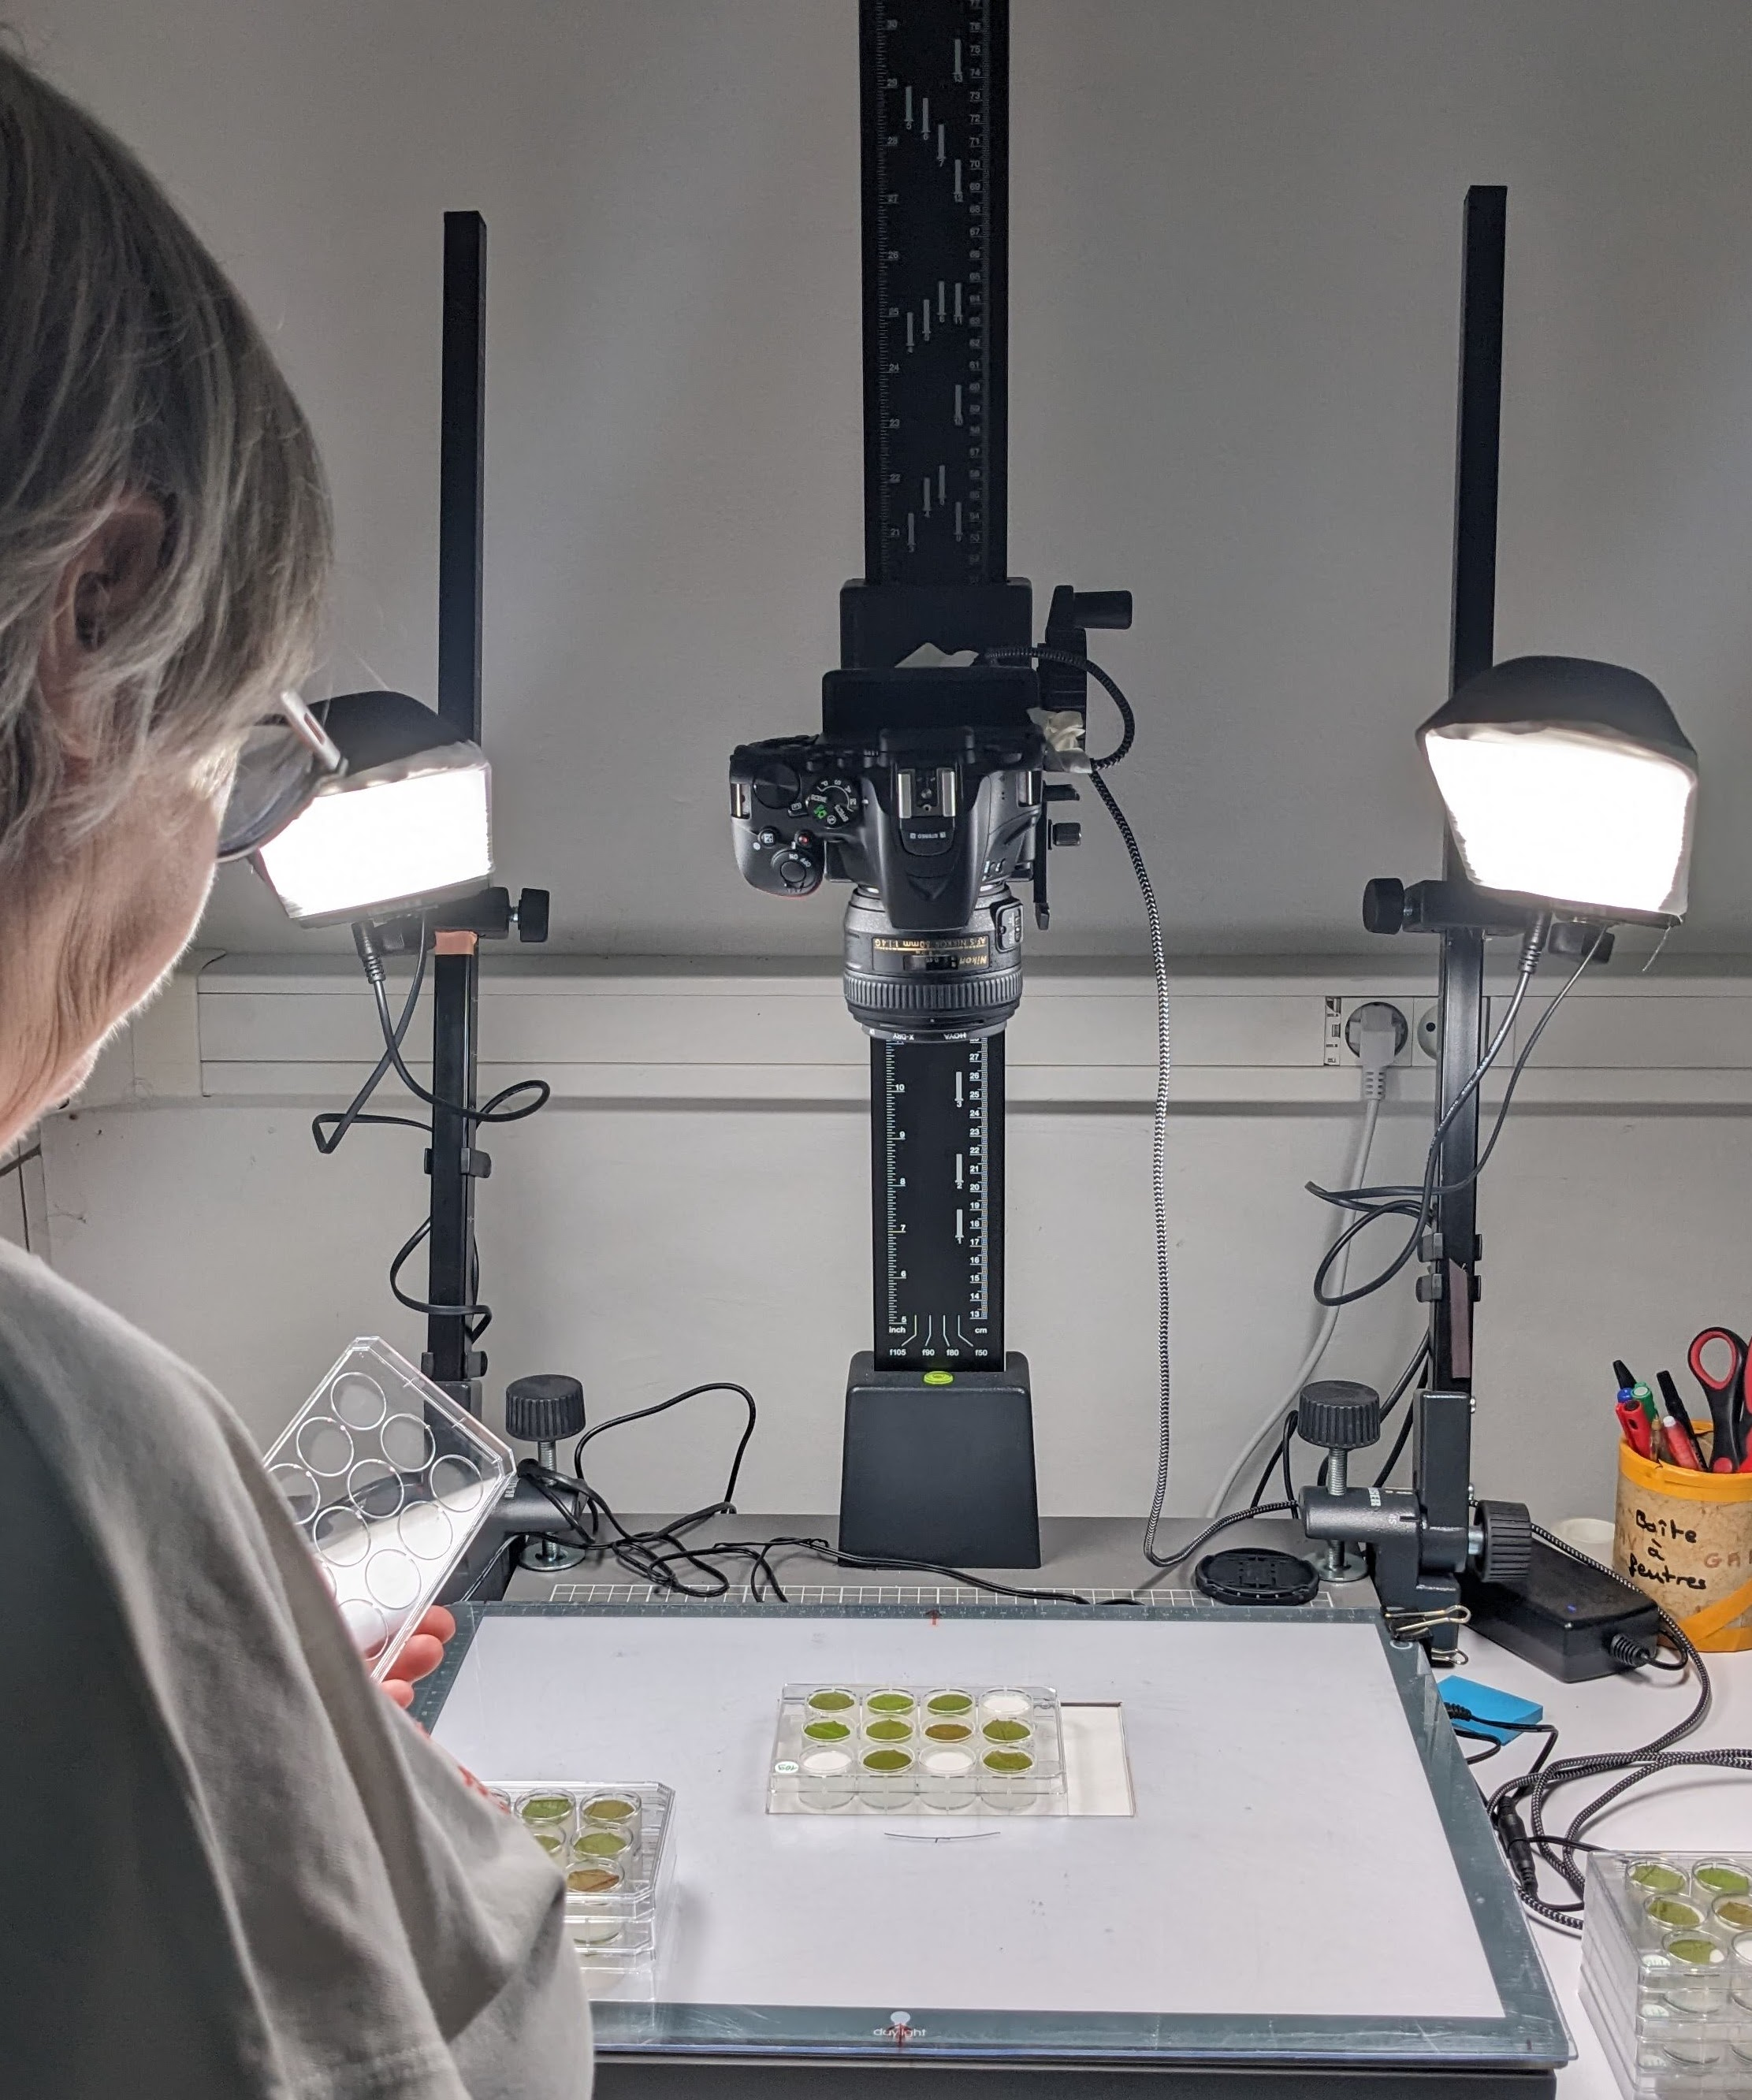
\includegraphics[width=0.5\linewidth]{2023_a_oiv_imaging_system.jpg}
        \caption{VEGOIA platform's manual imaging system}\label{fig:vegoia}
    \end{center}
\end{figure}

\begin{figure}[H]
    \centering
    \begin{subfigure}[b]{0.2\linewidth}
        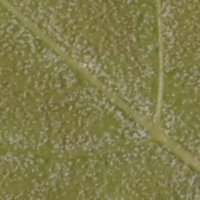
\includegraphics[width=\linewidth]{p_viticola/resources/images/2023_a_oiv_sporulation.png}
        \caption{Sporulation}\label{fig:sporulation}
    \end{subfigure}
    \begin{subfigure}[b]{0.2\linewidth}
        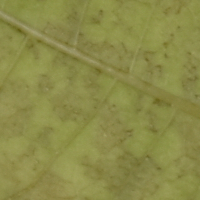
\includegraphics[width=\linewidth]{p_viticola/resources/images/2023_a_oiv_stains.png}
        \caption{Flecks}\label{fig:flecks}
    \end{subfigure}
    \begin{subfigure}[b]{0.2\linewidth}
        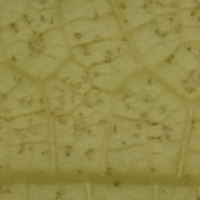
\includegraphics[width=\linewidth]{p_viticola/resources/images/2023_oiv_a_dots.png}
        \caption{Dots}\label{fig:dots}
    \end{subfigure}
    \begin{subfigure}[b]{0.2\linewidth}
        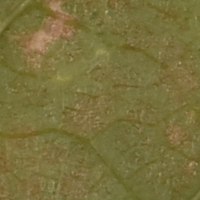
\includegraphics[width=\linewidth]{p_viticola/resources/images/2023_a_oiv_senescence.png}
        \caption{Senscence}\label{fig:senescence}
    \end{subfigure}
    \caption{Examples of \textit{Vitis} leaf discs infected with \textit{Plasmopara viticola} showing the four different phenotypes selected.}
\end{figure}

\begin{figure}[H]
    \centering
    \begin{subfigure}[b]{0.3\linewidth}
        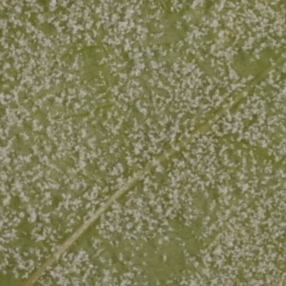
\includegraphics[width=\linewidth]{Exp21DM02_inoc2_T6_P35_a_4.png}
        \caption{OIV 1}\label{fig:issuegood}
    \end{subfigure}
    \begin{subfigure}[b]{0.3\linewidth}
        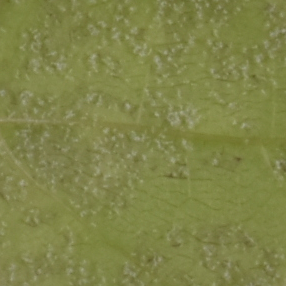
\includegraphics[width=\linewidth]{Exp20DM01_inoc2_T6_P01_c_3.png}
        \caption{OIV 3}\label{fig:issueblur}
    \end{subfigure}
    \begin{subfigure}[b]{0.3\linewidth}
        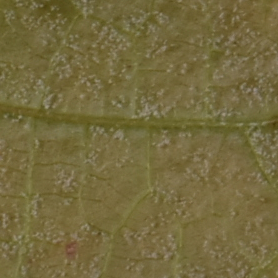
\includegraphics[width=\linewidth]{Exp21DM03_inoc3_T4_P32_c_1.png}
        \caption{OIV 5}\label{fig:issuecolor}
    \end{subfigure}
    \begin{subfigure}[b]{0.3\linewidth}
        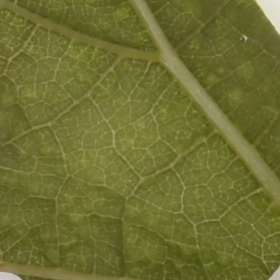
\includegraphics[width=\linewidth]{Exp21DM13_inoc2_T0_P34_b_1.png}
        \caption{OIV 7}\label{fig:issuecrop}
    \end{subfigure}
    \begin{subfigure}[b]{0.3\linewidth}
        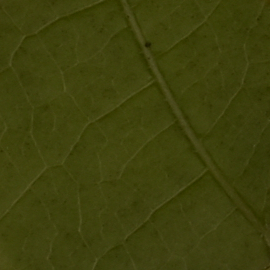
\includegraphics[width=\linewidth]{Exp21DM04_inoc2_T6_P02_c_1.png}
        \caption{OIV 9}\label{fig:issuedark}
    \end{subfigure}
    \begin{subfigure}[b]{0.3\linewidth}
        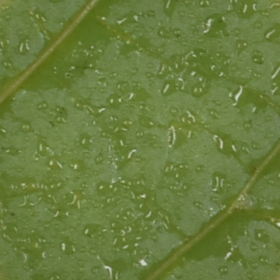
\includegraphics[width=\linewidth]{Exp22DM01_inoc1_T5_P03_a_1.png}
        \caption{OIV 9}\label{fig:issuewater}
    \end{subfigure}
    \caption{Examples of different issues present in the source images~\ref{fig:issuegood} represents a base good image. Some issues like darker images~\ref{fig:issuedark} can be fixed with pre-processing, others like color~\ref{fig:issuecolor}, crop~\ref{fig:issuecrop} and blur~\ref{fig:issueblur} are rare and can be discarded from the training . Finally images with water droplets~\ref{fig:issuewater} are very common enough that the model should be able to handle them.}
\end{figure}

\begin{table}[H]
\centering
\caption{Distribution of image quality and annotations for phenotype detecttion}
\label{tab:databincount}
\begin{tabular}{lrrrr}
\toprule
 issue &  sporulation &  necrosis\_dots &  necrosis\_stains &  necrosis\_senescence \\
\midrule
  blur &           11 &             10 &                2 &                    7 \\
colour &           23 &              0 &                0 &                   13 \\
  good &          983 &            579 &              261 &                  374 \\
 water &          102 &            118 &               25 &                   49 \\
 total &         1119 &            712 &              289 &                  444 \\
\bottomrule
\end{tabular}
\end{table}

\begin{figure}[H]
    \centering
    \begin{subfigure}[b]{0.3\linewidth}
        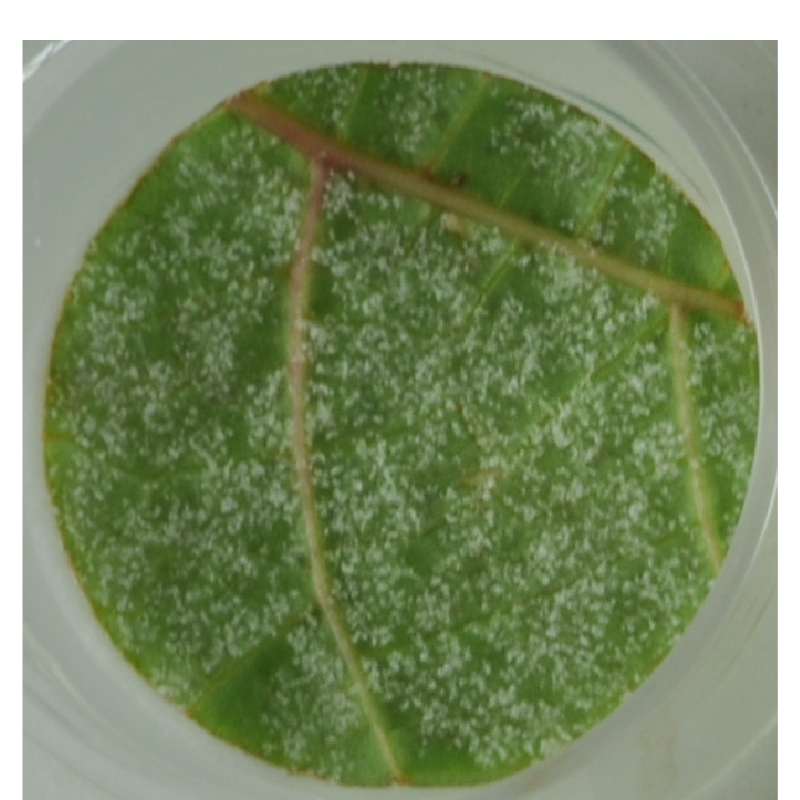
\includegraphics[width=\linewidth]{oiv1.png}
        \caption{OIV 1}\label{fig:oiv1}
    \end{subfigure}
    \begin{subfigure}[b]{0.3\linewidth}
        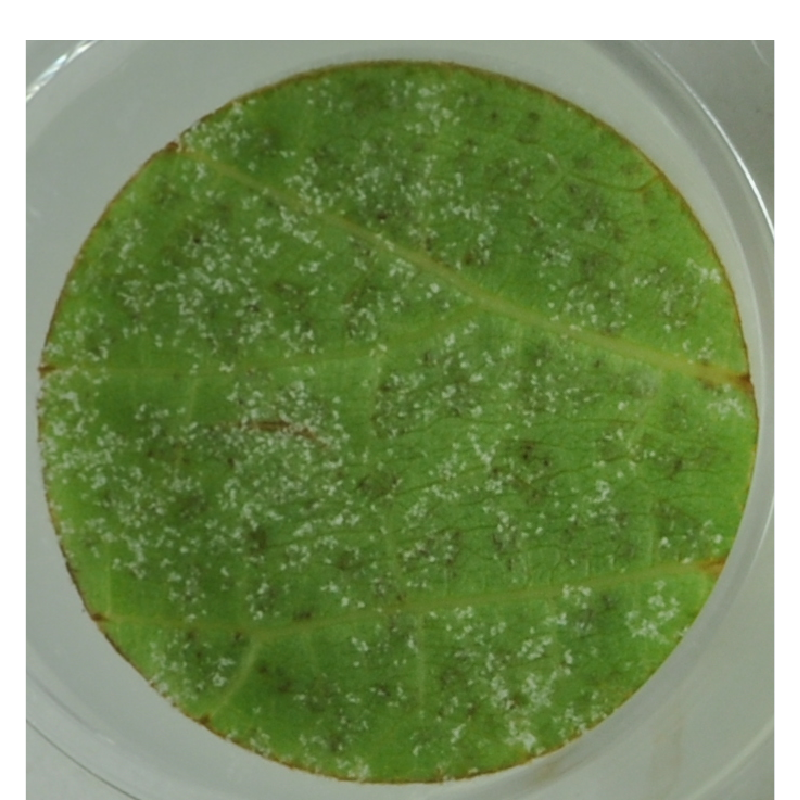
\includegraphics[width=\linewidth]{oiv3.png}
        \caption{OIV 3}\label{fig:oiv3}
    \end{subfigure}
    \begin{subfigure}[b]{0.3\linewidth}
        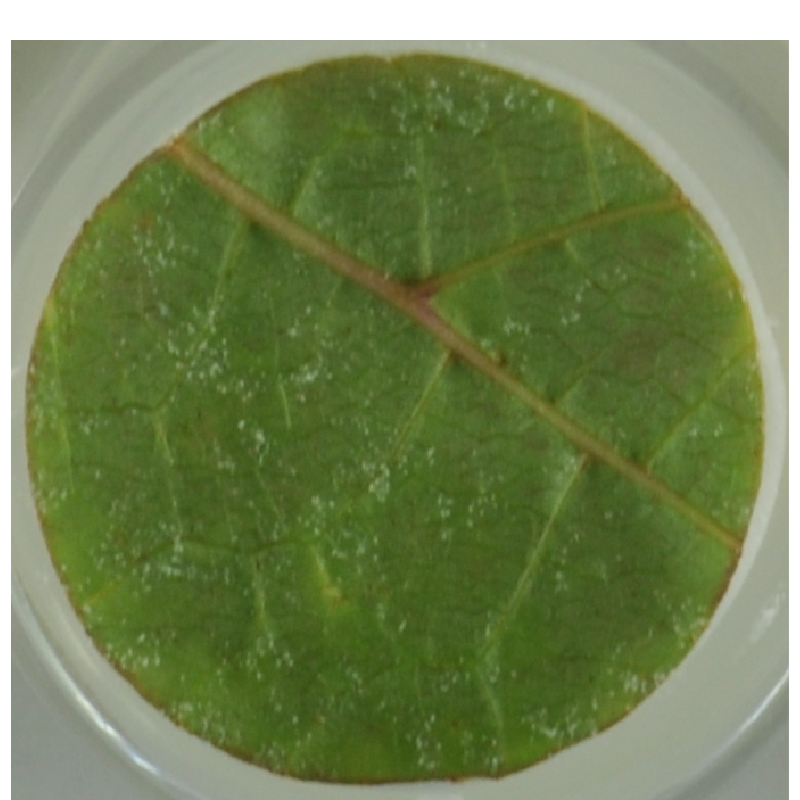
\includegraphics[width=\linewidth]{oiv5.png}
        \caption{OIV 5}\label{fig:oiv5}
    \end{subfigure}
    \begin{subfigure}[b]{0.3\linewidth}
        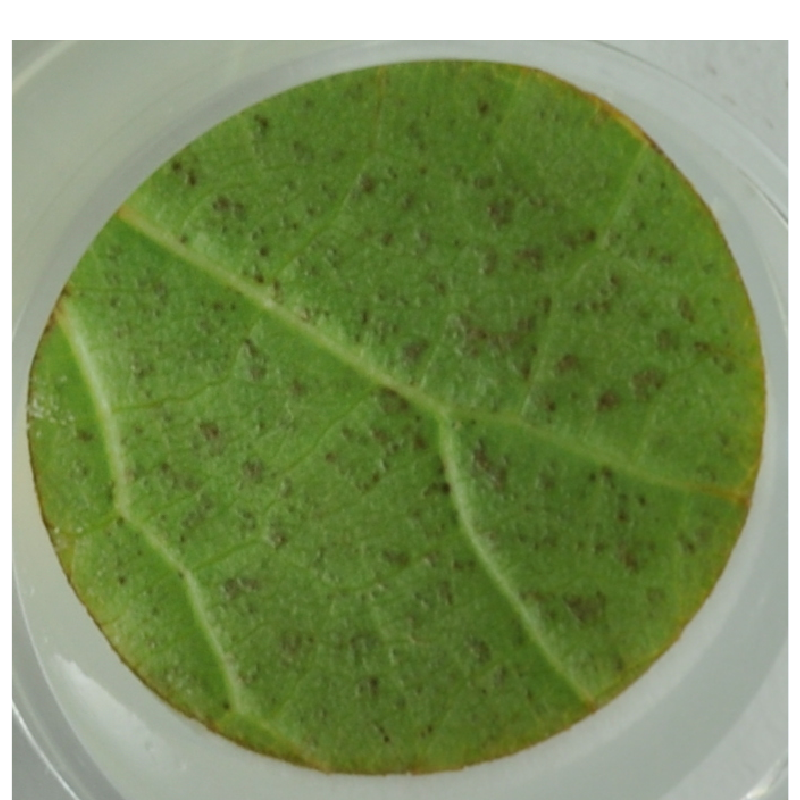
\includegraphics[width=\linewidth]{oiv7.png}
        \caption{OIV 7}\label{fig:oiv7}
    \end{subfigure}
    \begin{subfigure}[b]{0.3\linewidth}
        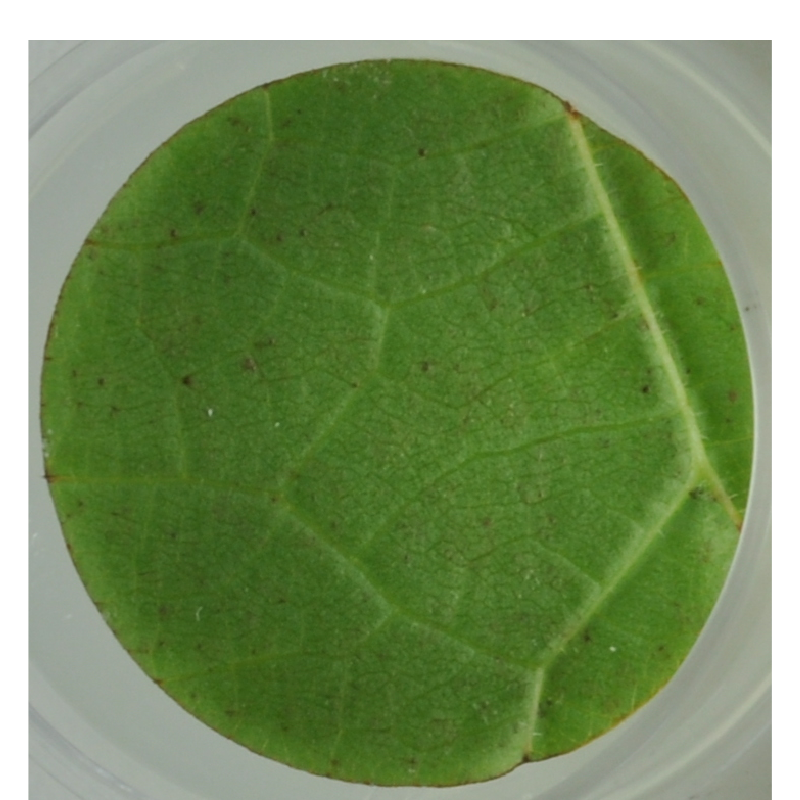
\includegraphics[width=\linewidth]{oiv9.png}
        \caption{OIV 9}\label{fig:oiv9}
    \end{subfigure}
    \caption{Examples of \textit{Vitis} leaf discs infected with \textit{Plasmopara viticola} annotated with OIV 452-1 values. Levels increase with resistance to pathogen. Upper row, susceptible leaf discs with levels 1 to 5. Lower row, resistant leaf disc~\ref{fig:oiv7} and fully resistant leaf disc~\ref{fig:oiv9}}\label{fig:phenotypes}
\end{figure}

\begin{table}[H]
\centering
\caption{Distribution of image quality and OIV values}
\label{tab:dataoivcount}
\begin{tabular}{rrrrrrrr}
\toprule
 oiv &  blur &  color &  crop &  dark &  good &  water &  total \\
\midrule
   1 &     0 &      0 &     3 &    10 &   626 &    116 &    755 \\
   3 &     2 &      2 &     0 &     7 &   479 &    144 &    634 \\
   5 &     3 &      1 &     0 &     5 &   412 &    146 &    567 \\
   7 &     1 &      0 &     3 &     6 &   549 &    141 &    700 \\
   9 &     0 &      0 &     4 &    12 &   513 &    331 &    860 \\
\bottomrule
\end{tabular}
\end{table}


\begin{figure}[H]
    \begin{center}
        \includegraphics[width=0.9\linewidth]{p_viticola/resources/images/leaf_disc_extraction_2.png}
        \caption{Leaf disc extraction workflow}\label{fig:preprocessing}
    \end{center}
\end{figure}


\begin{equation}
    L = -\sum_{c=1}^My_{o,c}\log(p_{o,c})\label{fml:crossentropy}
\end{equation}

\begin{figure}[H]
    \centering
    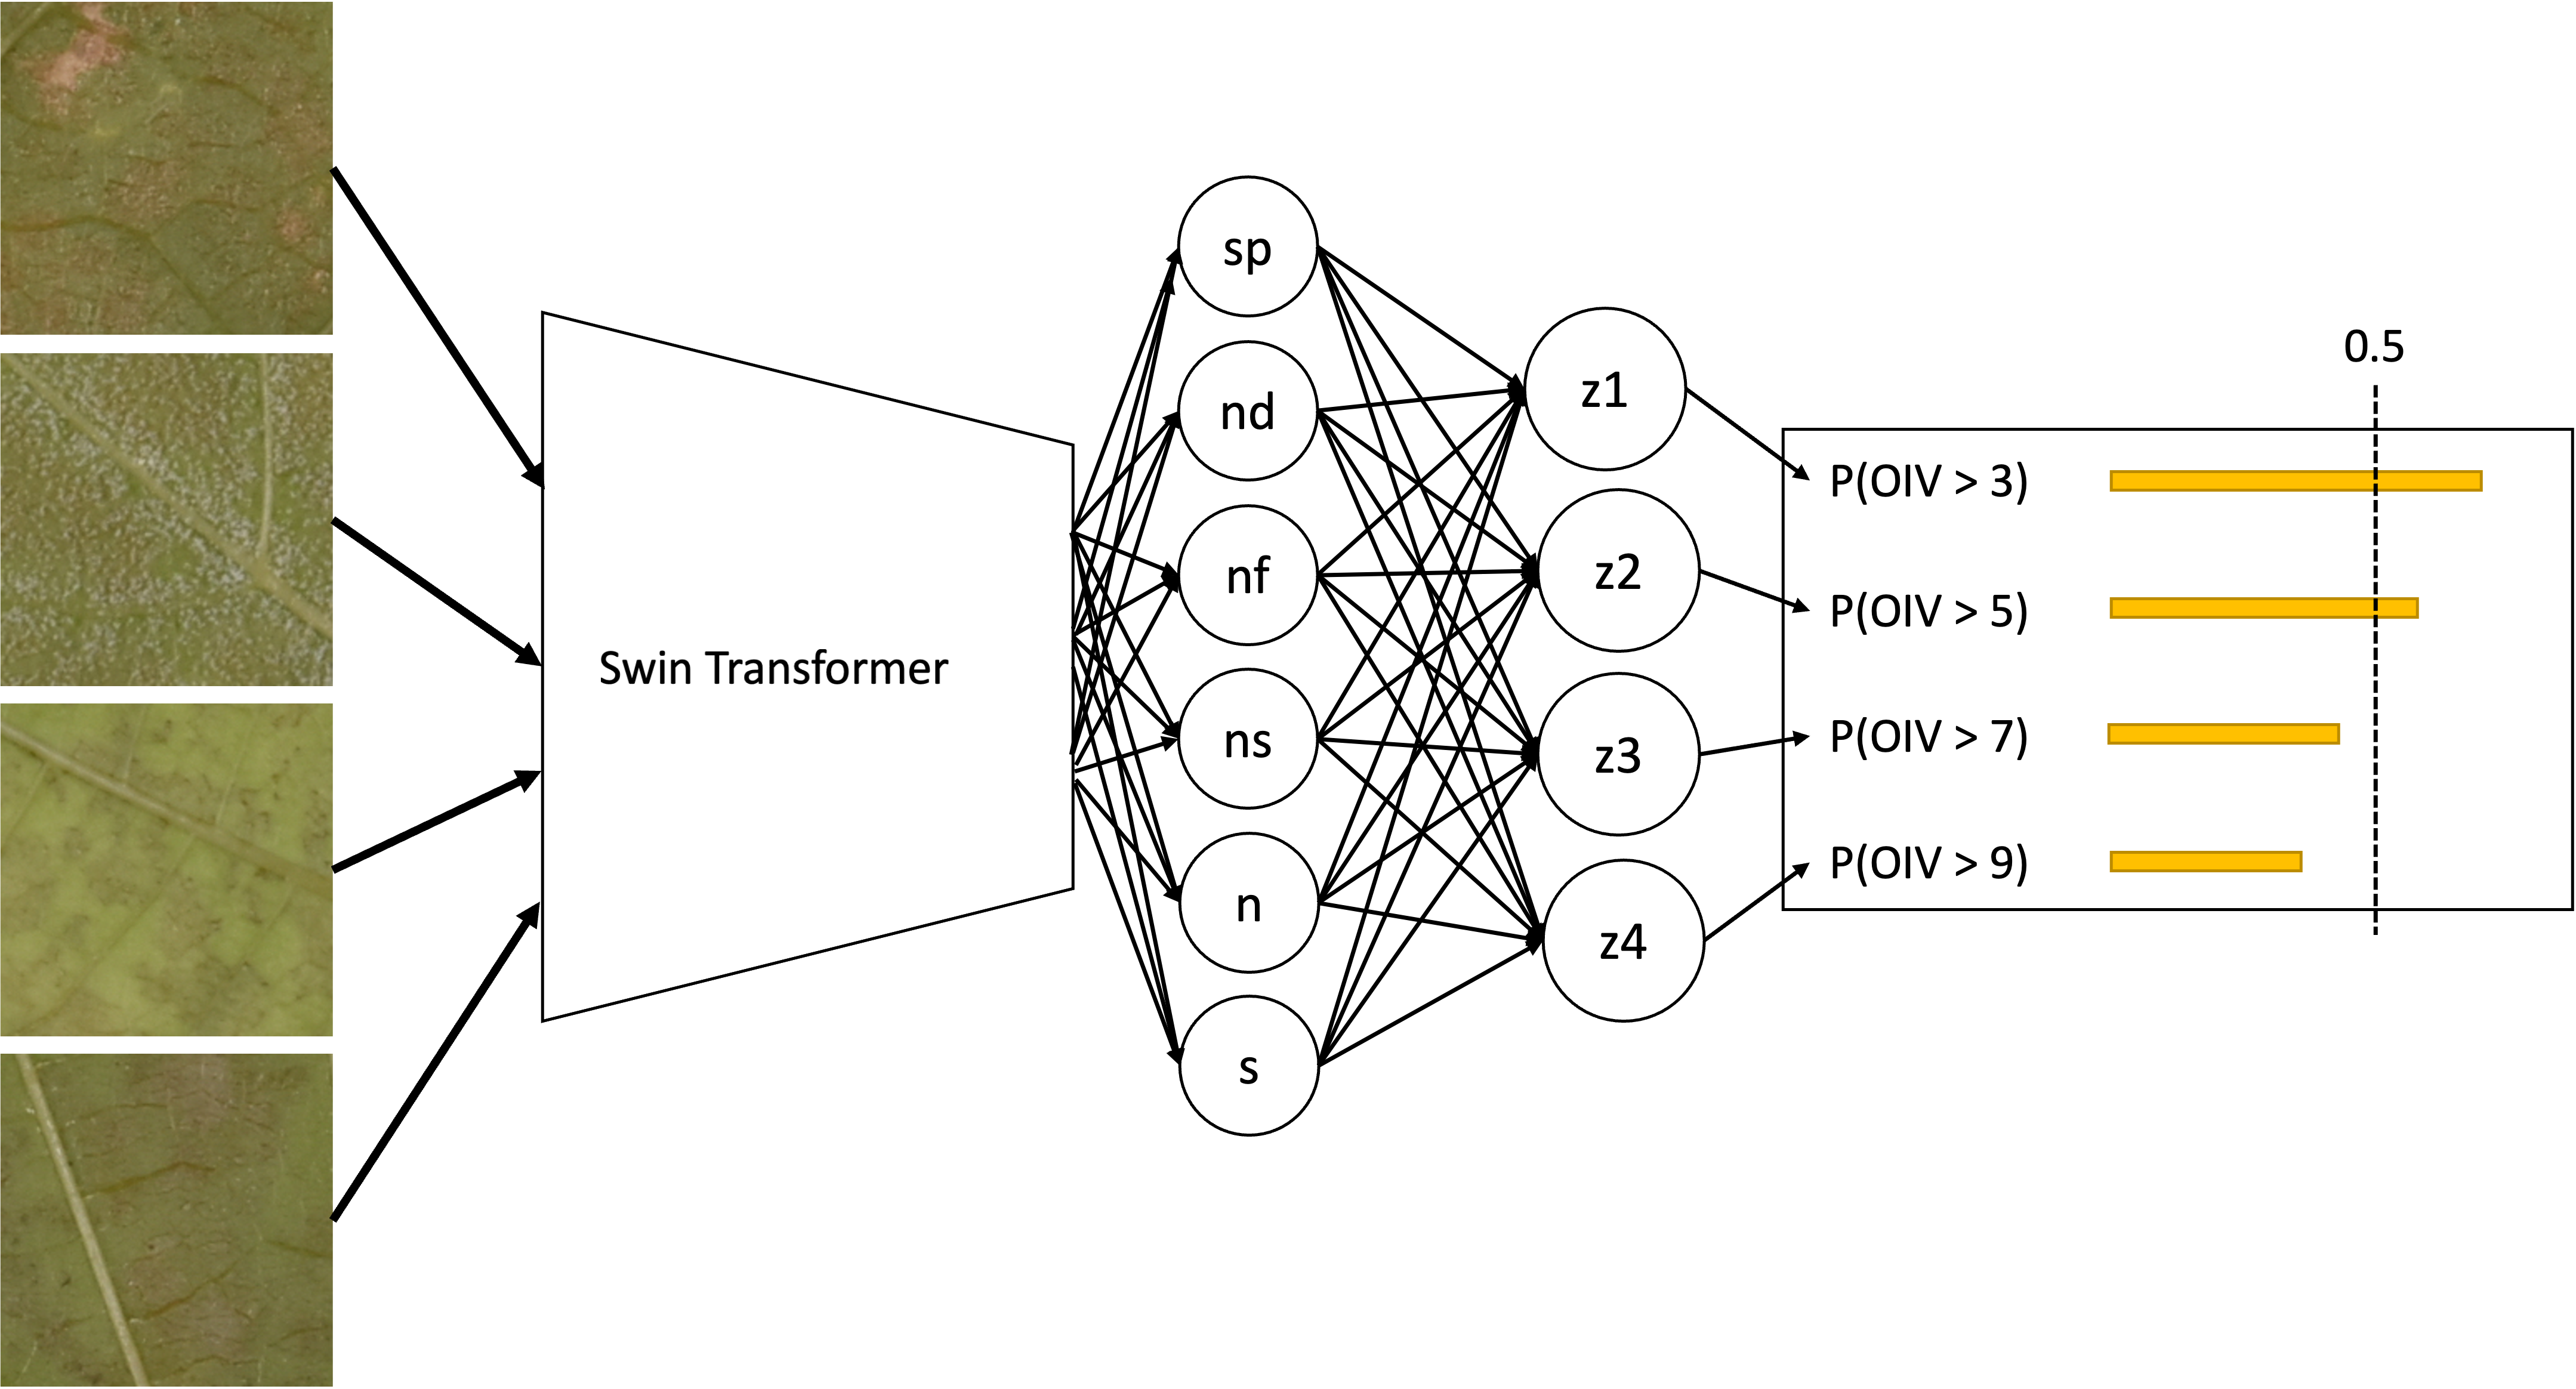
\includegraphics[width=0.9\linewidth]{p_viticola/resources/images/2023_a_oiv_bin_corn.png}
    \caption{Rank-consistent ordinal regression (CORN) architecture with output example predicting OIV 7}
    \label{fig:corn}
\end{figure}

\begin{equation}
    f(x^{[i]}) = \hat{P}(y^{[i]} > r_{k}|y^{[i]} > r_{k-1})\label{fml:binclass}
\end{equation}

\begin{equation}
    \hat{P}(y^{[i]} > r_{k}) = \prod_{j=1}^{k}f_{j}(x^{[i]})\label{fml:unconditionalprob}
\end{equation}

\begin{equation}
    OIV = (\sum_{j=1}^{K-1}\mathbb{1}(\hat{P}(y^{[i]} > r_{j}) > 0.5))*2 + 1\label{fml:rankprob}
\end{equation}

\section{Results and Discussion}

\subsection{Leaf Disc Detection}

\begin{table}[H]
\centering
\caption{Leaf disc detection models evaluation}
\label{tab:leafdiscdetectionresult}
\begin{tabular}{lrrrrr}
\toprule
{} & \multicolumn{5}{l}{val\_loss} \\
{} &    count &    min &    mean & median &         std \\
scheduler &          &        &         &        &             \\
\midrule
None      &       20 &  0.015 &  0.0176 &  0.017 &  0.00223371 \\
steplr    &       15 &  0.012 &  0.0154 &  0.015 &  0.00213140 \\
\bottomrule
\end{tabular}
\end{table}

\subsection{Binary Predictions}

Phenotypes legend:
\begin{itemize}
    \item sp = sporulation
    \item nd = necrosis dots
    \item nf = necrosis flecks
    \item ns = necrosis stains
    \item n = necrosis, all types
    \item s = stains, flecks or senescence
\end{itemize}

\begin{table}[H]
\centering
\caption{Results for binary pheotype detection}
\label{tab:binres}
\begin{tabular}{lrl}
\toprule
          phenotypes &  max training epochs & F1 weighted average \\
\midrule
               sp, n &                    5 &          0.87\textpm0.028 \\
               sp, n &                   10 &          0.89\textpm0.008 \\
               sp, n &                   20 &          0.90\textpm0.008 \\
               sp, n &                  200 &          0.90\textpm0.007 \\
      sp, nd, nf, ns &                    5 &          0.82\textpm0.031 \\
      sp, nd, nf, ns &                   10 &          0.86\textpm0.007 \\
      sp, nd, nf, ns &                   20 &          0.87\textpm0.010 \\
      sp, nd, nf, ns &                  200 &          0.88\textpm0.008 \\
sp, nd, nf, ns, n, s &                    5 &          0.81\textpm0.040 \\
sp, nd, nf, ns, n, s &                   10 &          0.85\textpm0.014 \\
sp, nd, nf, ns, n, s &                   20 &          0.88\textpm0.011 \\
sp, nd, nf, ns, n, s &                  200 &          0.88\textpm0.008 \\
           sp, nd, s &                    5 &          0.84\textpm0.011 \\
           sp, nd, s &                   10 &          0.87\textpm0.005 \\
           sp, nd, s &                   20 &          0.88\textpm0.006 \\
           sp, nd, s &                  200 &          0.89\textpm0.007 \\
\bottomrule
\end{tabular}
\end{table}

\subsection{OIV prediction}

\begin{table}[H]
\centering
\caption{Results for OIV 452-1 ordinal regression}
\label{tab:oivres}
\begin{tabular}{rlll}
\toprule
 backbone max training epochs &  backbone phenotypes &        mae &        mse \\
\midrule
                            5 &       sp, nd, nf, ns & 0.18\textpm0.014 & 0.19\textpm0.014 \\
                           10 &       sp, nd, nf, ns & 0.18\textpm0.011 & 0.20\textpm0.024 \\
                           20 &       sp, nd, nf, ns & 0.18\textpm0.003 & 0.19\textpm0.008 \\
                          200 &       sp, nd, nf, ns & 0.18\textpm0.011 & 0.19\textpm0.024 \\
                            5 & sp, nd, nf, ns, n, s & 0.17\textpm0.006 & 0.18\textpm0.007 \\
                           10 & sp, nd, nf, ns, n, s & 0.18\textpm0.007 & 0.19\textpm0.010 \\
                           20 & sp, nd, nf, ns, n, s & 0.19\textpm0.005 & 0.20\textpm0.014 \\
                          200 & sp, nd, nf, ns, n, s & 0.18\textpm0.002 & 0.20\textpm0.006 \\
                            5 &            sp, nd, s & 0.18\textpm0.009 & 0.19\textpm0.016 \\
                           10 &            sp, nd, s & 0.44\textpm0.407 & 1.02\textpm1.502 \\
                           20 &            sp, nd, s & 0.19\textpm0.016 & 0.20\textpm0.018 \\
                          200 &            sp, nd, s & 0.50\textpm0.328 & 0.93\textpm0.909 \\
\bottomrule
\end{tabular}
\end{table}

\begin{table}[H]
\centering
\caption{Validation dataset confusion matrix, MSE:0.175}
\label{tab:oivcm}
\begin{tabular}{lrrrrr}
\toprule
{} &    0 &   1 &   2 &   3 &    4 \\
\midrule
0 &  101 &  12 &   0 &   0 &    0 \\
1 &   16 &  77 &   1 &   0 &    0 \\
2 &    0 &  11 &  69 &   2 &    1 \\
3 &    0 &   0 &   7 &  72 &   25 \\
4 &    0 &   0 &   0 &  13 &  111 \\
\bottomrule
\end{tabular}
\end{table}


\section{Never Seen Experiment}

\begin{figure}[H]
    \centering
    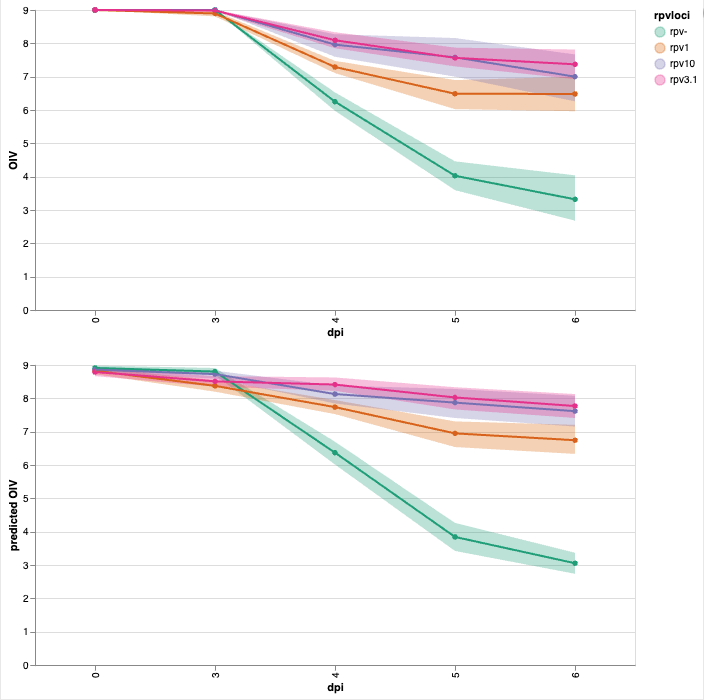
\includegraphics[width=0.8\linewidth]{p_viticola//resources//images/cmp_2023_oiv_evo.png}
    \caption{Predicted OIV 452-1 versus annotated one when following pathogen evolution}
    \label{fig:newexpprog}
\end{figure}


\begin{figure}[H]
    \centering
    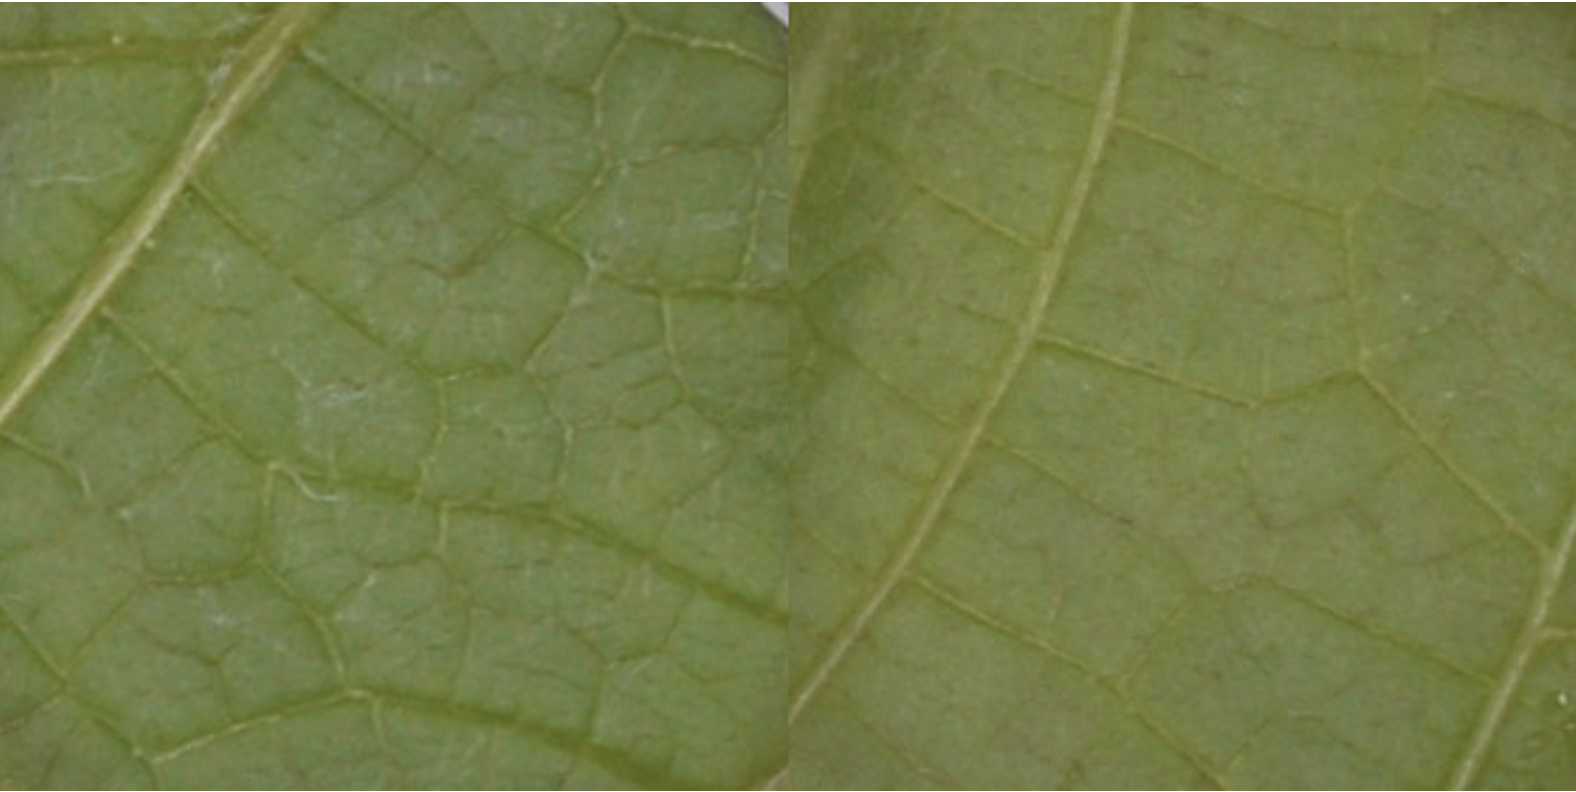
\includegraphics[width=0.5\linewidth]{p_viticola//resources//images/nexexppatcherror.png}
    \caption{Leaf discs annotated with OIV 9 erroneously predicted as OIV 7}
    \label{fig:newexperror}
\end{figure}


\begin{table}[H]
\centering
\caption{ANOVA for annotated data}
\label{tab:oivannova}
\begin{tabular}{lrrrr}
\toprule
{} &      sum\_sq &     df &          F &        PR(>F) \\
\midrule
C(rpvloci) &  716.93 &    8 &  37.01 &  2.66e-38 \\
Residual   &  600.45 &  248 &        NaN &           NaN \\
\bottomrule
\end{tabular}
\end{table}

\begin{table}[H]
\centering
\caption{ANOVA for predicted data}
\label{tab:poivannova}
\begin{tabular}{lrrrr}
\toprule
{} &      sum\_sq &     df &          F &        PR(>F) \\
\midrule
C(rpvloci) &  872.63 &    8 &  47.27 &  9.90e-46 \\
Residual   &  572.28 &  248 &        NaN &           NaN \\
\bottomrule
\end{tabular}
\end{table}

\section{Conclusions and perspectives}




\end{document}